
\documentclass[a4paper,12pt]{article}

\usepackage{graphicx} % Required for inserting images
\usepackage{amsmath,amssymb,amsfonts}
\usepackage{subcaption}
% -----------------------
% Package Imports
% -----------------------

% Set page margins
\usepackage[a4paper, top=1in, bottom=0.8in, left=1.1in, right=0.8in]{geometry}

% Use Times New Roman font
\usepackage{times}

% Add page numbering
\pagestyle{plain}

% Enable graphics inclusion
\usepackage{graphicx}
\usepackage{float}
% Enable code listings
\usepackage{listings}
\usepackage{xcolor} % For customizing code colors
\setlength{\parindent}{0pt}




\begin{document}
	\section{Experiment No. 1}
	
	\section{Experiment Title }
	
	Introduction to different DC and AC Machines and General discussion on Safety and Precautions
	
	\section{Objective}
	
	The objectives of this lab are as follows:
	\begin{itemize}
    \item To examine and document the specifications of various electrical equipment and training modules.
\item To identify the functions and operational parameters of the provided devices.
\item To ensure proper handling and safety measures while working with electrical components.
\item To analyze the role of each module in electrical circuit training and practical applications.
\item To develop an understanding of measurement techniques and data recording for future experiments.
	\end{itemize}
	
	\section{Theory}
A machine is a device that uses energy to perform a specific task. It can be mechanical, electrical, or a combination of both. Machines typically convert one form of energy into another to accomplish work.In the context of your lab report, DC and AC machines refer to electrical machines that either convert electrical energy into mechanical energy (motors) or mechanical energy into electrical energy (generators). Transformers, which modify voltage levels, are also considered AC machines.
	
	\section{Types of DC and AC Machines}
	
	\subsection{DC Machines}
	DC machines are commonly used in applications requiring variable speed control and high starting torque. They are classified into:
	\begin{enumerate}
		\item \textbf{DC Motors}: Convert electrical energy into mechanical energy.
		\item \textbf{DC Generators}: Convert mechanical energy into electrical energy.
	\end{enumerate}
	Based on excitation, DC machines are further classified as:
	\begin{enumerate}
		\item Separately excited DC machines
		\item Shunt-wound DC machines
		\item Series-wound DC machines
		\item Compound-wound DC machines
	\end{enumerate}
	\newpage
	
	\begin{figure}[H]
		\centering
		\includegraphics[width=.7\linewidth, height=0.2\textheight]{"Images/5"}
		\caption{Complete Experimental Setup}
	\end{figure}
	
	\subsection{AC Machines}
	AC machines are widely used due to their efficiency and robustness. They are classified into:
	\begin{enumerate}
		\item \textbf{Induction Machines}: Work on the principle of electromagnetic induction.
		\item \textbf{Synchronous Machines}: Operate at a constant speed determined by the supply frequency.
	
	\end{enumerate}
	
	\section{Description of Machines}
	
	\subsection{DC Motor and Generator}
	A universal motor is a type of electric motor that can operate on both AC and DC power supplies. It is commonly found in household appliances like mixers and drills.
	\begin{figure}[H]
		\centering
		\includegraphics[width=.7\linewidth, height=0.2\textheight]{"Images/6"}
		\caption{DC Motor and Generator}
	\end{figure}
	
	% DC Machine Specifications
	\subsubsection{DC Motor Specifications}
	\begin{table}[H]
		\centering
		\caption{DC Motor Specifications}
		\begin{tabular}{| c | c |}
			\hline
			\textbf{Specification} & \textbf{Value} \\ \hline
			Power Rating & 300 W\\ \hline
			Voltage Rating [EXC.SERIES \& EXC. SEP] & 220 V \\ \hline
			Current Rating [EXC SERIES] & 1.9 A \\ \hline
			Current Rating [EXC SEP] & 1.8 A \\ \hline
			Vexc & 220 V \\ \hline
			Iexc & 0.1 A \\ \hline
			Speed & 2500 RPM \\ \hline
			
		\end{tabular}
		
		
		\label{tab:2}
	\end{table}
	
	% DC Generator Specifications
	\subsubsection{DC Generator Specifications}
	\begin{table}[H]
		\centering
		\caption{DC Generator}
		\begin{tabular}{| c | c |}
			\hline
			\textbf{Specification} & \textbf{Value} \\ \hline
			Power Rating & 300 W\\ \hline
			Voltage Rating [EXC.SERIES] & 210 V \\ \hline
			Voltage Rating [ EXC. COMP] & 220 V \\ \hline
			Current Rating [EXC SERIES \& EXC COMP] & 1.4 A \\ \hline
			Vexc & 0-220 V \\ \hline
			Iexc & 0.11 A \\ \hline
			Speed & 3000 RPM \\ \hline
			
		\end{tabular}
		
		\label{tab:2}
	\end{table}

	\subsection{Three-Phase Asynchronous Motor}
	A three-phase asynchronous motor, also known as an induction motor, operates on the principle of electromagnetic induction. It is widely used in industrial applications due to its robustness and self-starting capability.
	\begin{figure}[H]
		\centering
			\includegraphics[width=.7\linewidth, height=0.25\textheight]{"Images/7"}
		\caption{Three-Phase Asynchronous Motor}
		
	\end{figure}
	\subsubsection{Specifications of Three-Phase Asynchronous Motor}

\begin{table}[H]
	\centering
	\caption{Three-Phase Asynchronous Motor Specifications}
		\scalebox{.92}{
		
		\begin{tabular}{|l|c|c|c|c|c|c|}
			\hline
			\textbf{Type} & \textbf{Power (W)} & \textbf{Speed (rpm)} & \textbf{Voltage (V)} & \textbf{Current (A)} & \textbf{Frequency (Hz)} & \textbf{Poles} \\
			\hline
			Star Connection  & 500  & 2850  & 400  & 1.5  & 50  & 2  \\ \hline
			Delta Connection  & 500  & 2850  & 230  & 2.6  & 50  & 2  \\ \hline
		\end{tabular}
	}
\end{table}


	\subsection{Three-Phase Synchronous Motor}
	A three-phase synchronous motor runs at a constant speed determined by the supply frequency. It requires external excitation and is commonly used in applications requiring precise speed control.
		\begin{figure}[H]
			\caption{Power Supply Specifications}
		\centering
		\includegraphics[width=.6\linewidth, height=0.2\textheight]{"Images/8"}
		\caption{Three-Phase Synchronous Motor}
		
	\end{figure}
		\subsubsection{Specifications of Three-Phase Synchronous Motor}
\begin{table}[H]
	\centering
	\caption{Three-Phase Synchronous Motor Specifications}
		\begin{tabular}{|l|c|c|c|c|c|c|c|}
		
		\hline
		\textbf{Type} & \textbf{Power} & \textbf{Speed} & \textbf{Voltage} & \textbf{Current} & \textbf{cos $\phi$} & \textbf{Exc. Volt.} & \textbf{Exc. Curr.} \\
		& (W) & (rpm) & (V) & (A) & & (V) & (A) \\
		\hline
		Star  & 350  & 3000  & 400  & 0.7  & 1  & 220  & 0.45  \\ \hline
		Delta  & 350  & 3000  & 230  & 1.2  & 1  & 220  & 0.45  \\ \hline
	\end{tabular}
\end{table}


	\newpage
	\subsection{Universal Motor}
	A universal motor is a type of electric motor that can operate on both AC and DC power supplies. It is commonly found in household appliances like mixers and drills.
	\begin{figure}[H]
		\centering
		\includegraphics[width=.7\linewidth, height=0.2\textheight]{"Images/9"}
		\caption{Universal Motor}
	\end{figure}
	\subsubsection{Specifications of Universal Motor}
	\begin{table}[h]
		\centering
		\caption{Specifications of Universal Motor}
		\begin{tabular}{|l|c|c|c|c|}
				\hline
			\textbf{Type} & \textbf{Power (W)} & \textbf{Speed (rpm)} & \textbf{Voltage (V)} & \textbf{Current (A)} \\
			\hline
			AC Operation  & 450  & 3750  & 230  & 4.4  \\ 	\hline
			DC Operation  & 365  & 3050  & 220  & 2.6  \\ 	\hline
		
		\end{tabular}
		\label{tab:universal_motor_specs}
	\end{table}
	\subsection{Tachogenerator}
	A tachogenerator is a device used to measure the rotational speed of a shaft. It converts mechanical motion into a proportional electrical signal.
		\begin{figure}[H]
		\centering
		\includegraphics[width=.5\linewidth, height=0.2\textheight]{"Images/13"}
		\caption{Tachogenerator}
	\end{figure}
	
	\begin{table}[H]
		\centering
		\caption{Universal Motor Specifications}
		\begin{tabular}{|l|c|c|c|}
		\hline
		\textbf{Voltage Constant} & \textbf{Voltage (V)} & \textbf{Speed (rpm)} & \textbf{Current (A)} \\
		\hline
		0.06 V/rev & 300 & 5000 & 0.07 \\ \hline
		2 mV/rev   & 10  & 5000 & 0.07 \\ \hline
	\end{tabular}
	\end{table}

	
	\subsection{AC-DC Multimeter}
	An AC-DC multimeter is an instrument used to measure voltage, current, and resistance in both AC and DC circuits.
	\begin{figure}[H]
		\centering
		\begin{subfigure}[t]{.32\textwidth}
			\centering
			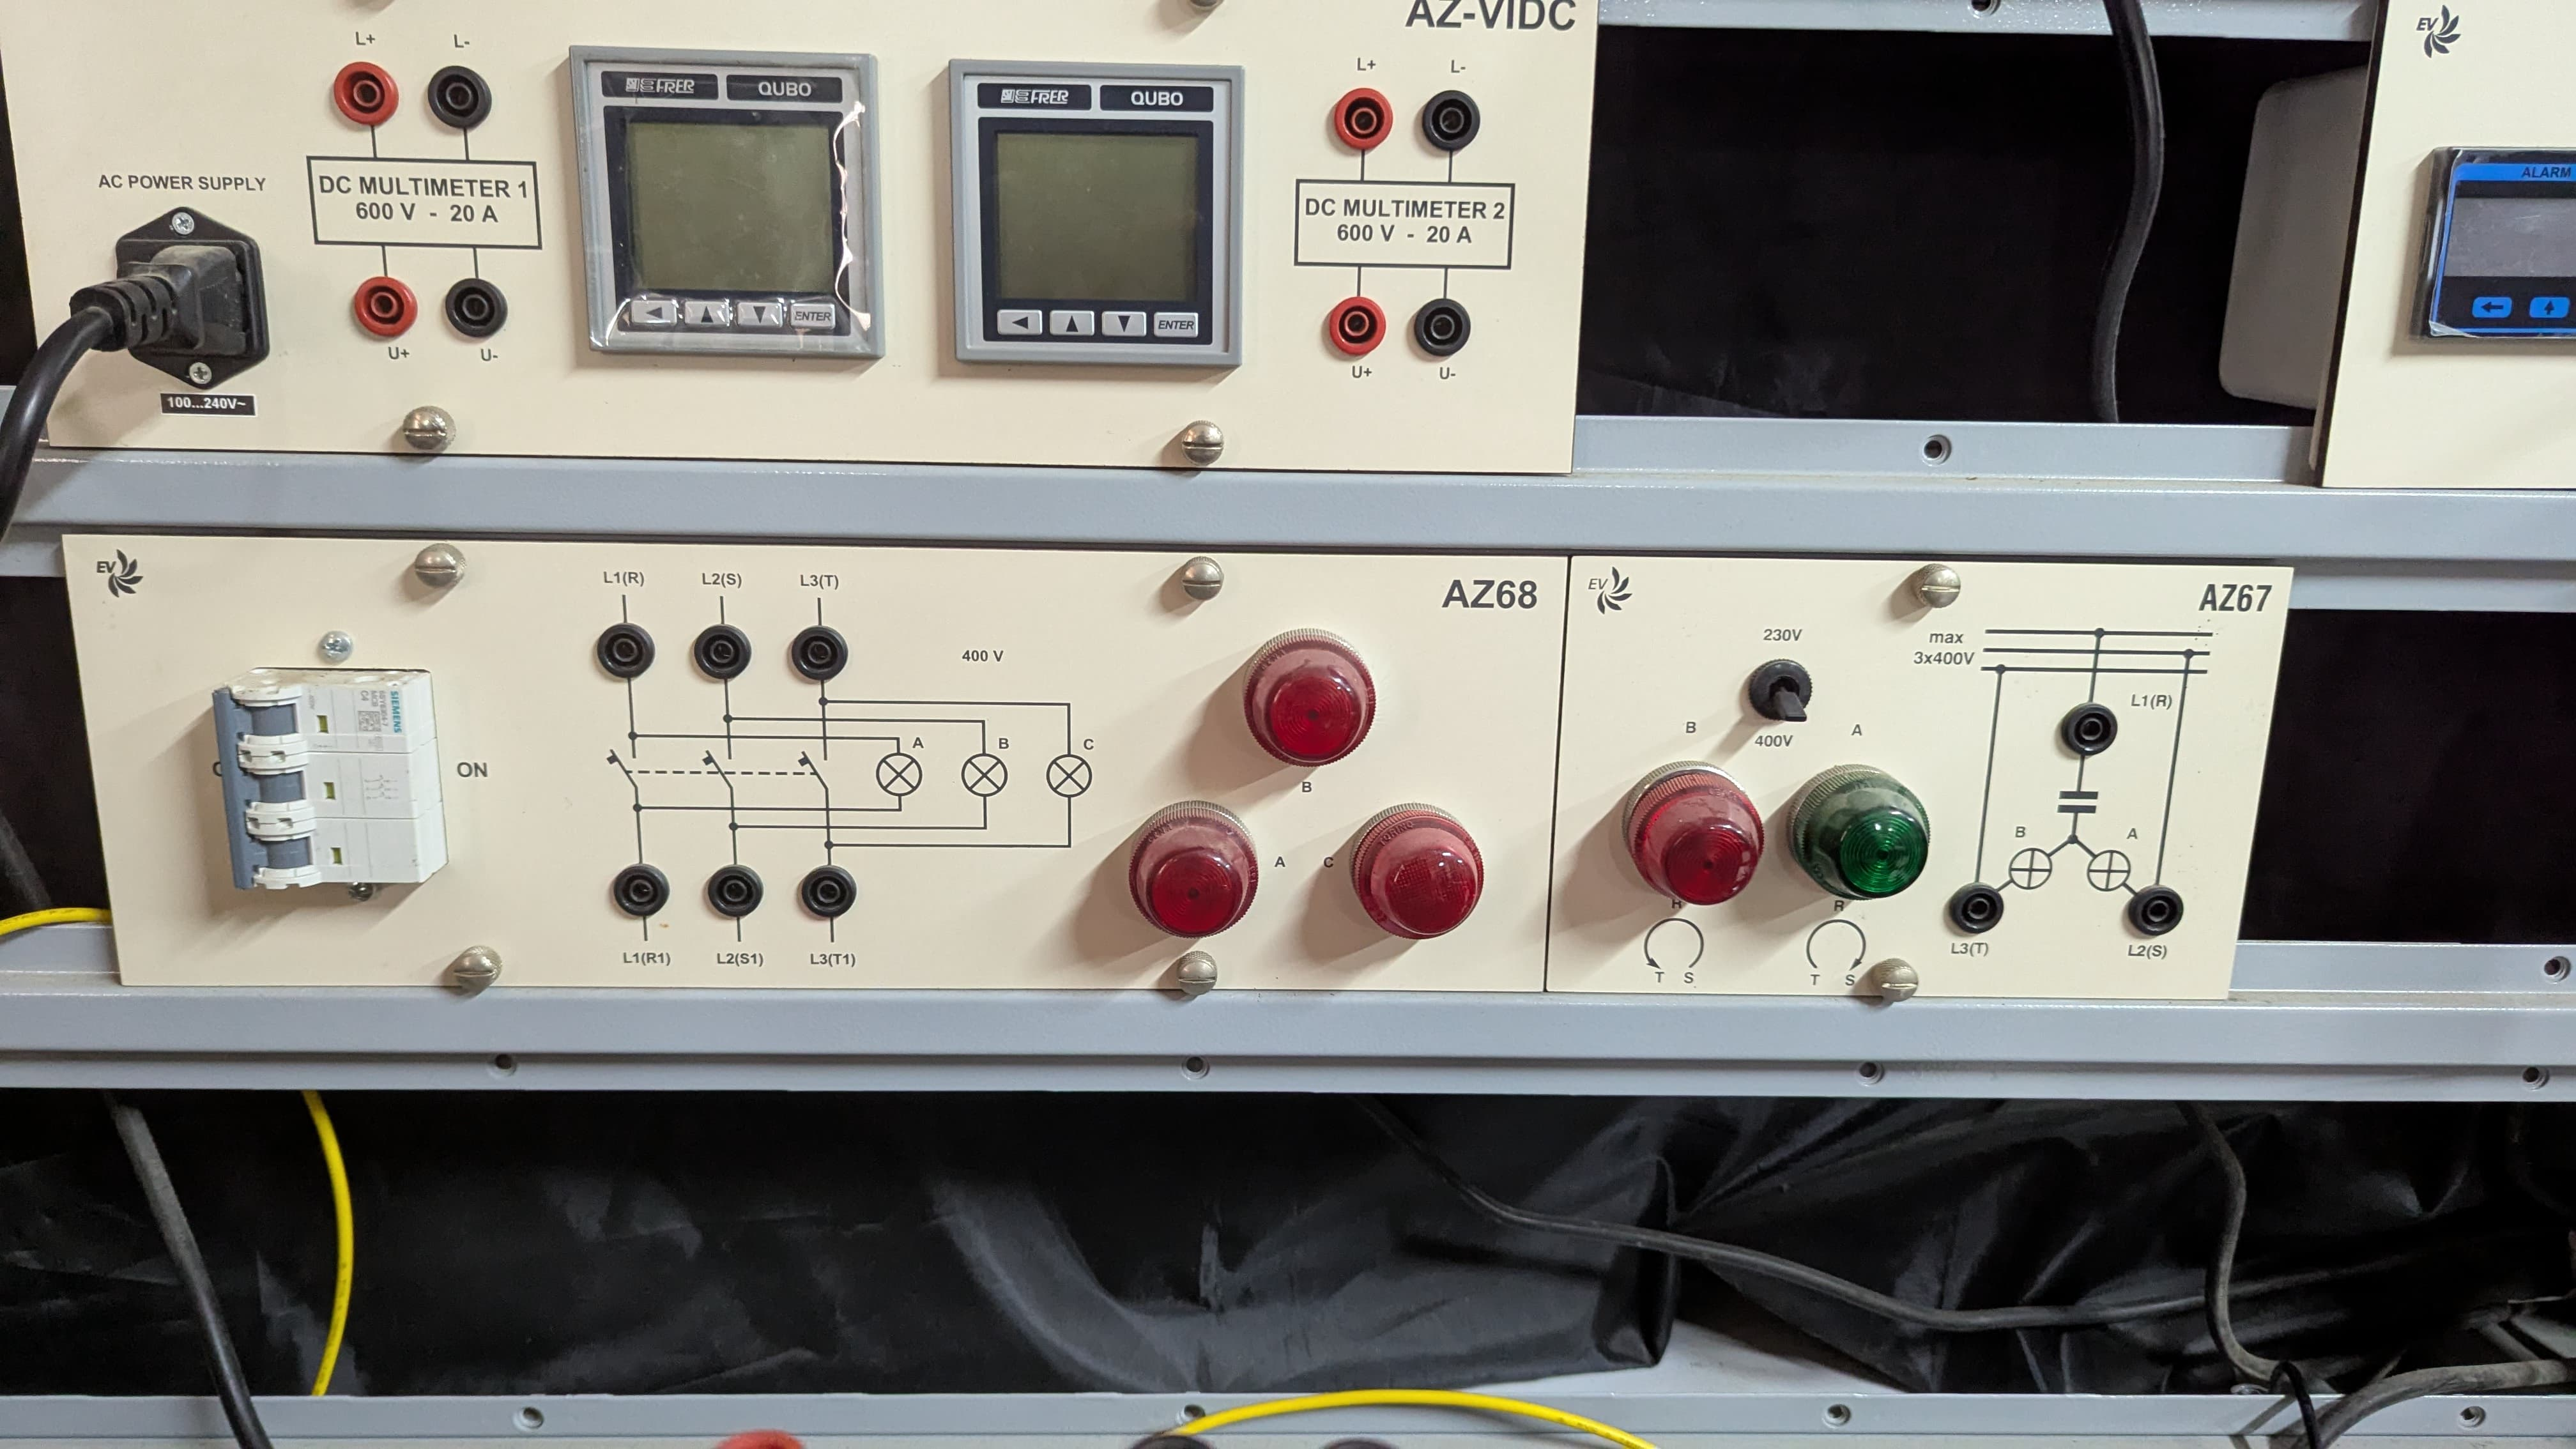
\includegraphics[width=1\linewidth]{Images/15}
			\caption{ }
			\vspace{0.1cm}
		\end{subfigure}
		\hfill
		\begin{subfigure}[t]{.32\textwidth}
			\centering
			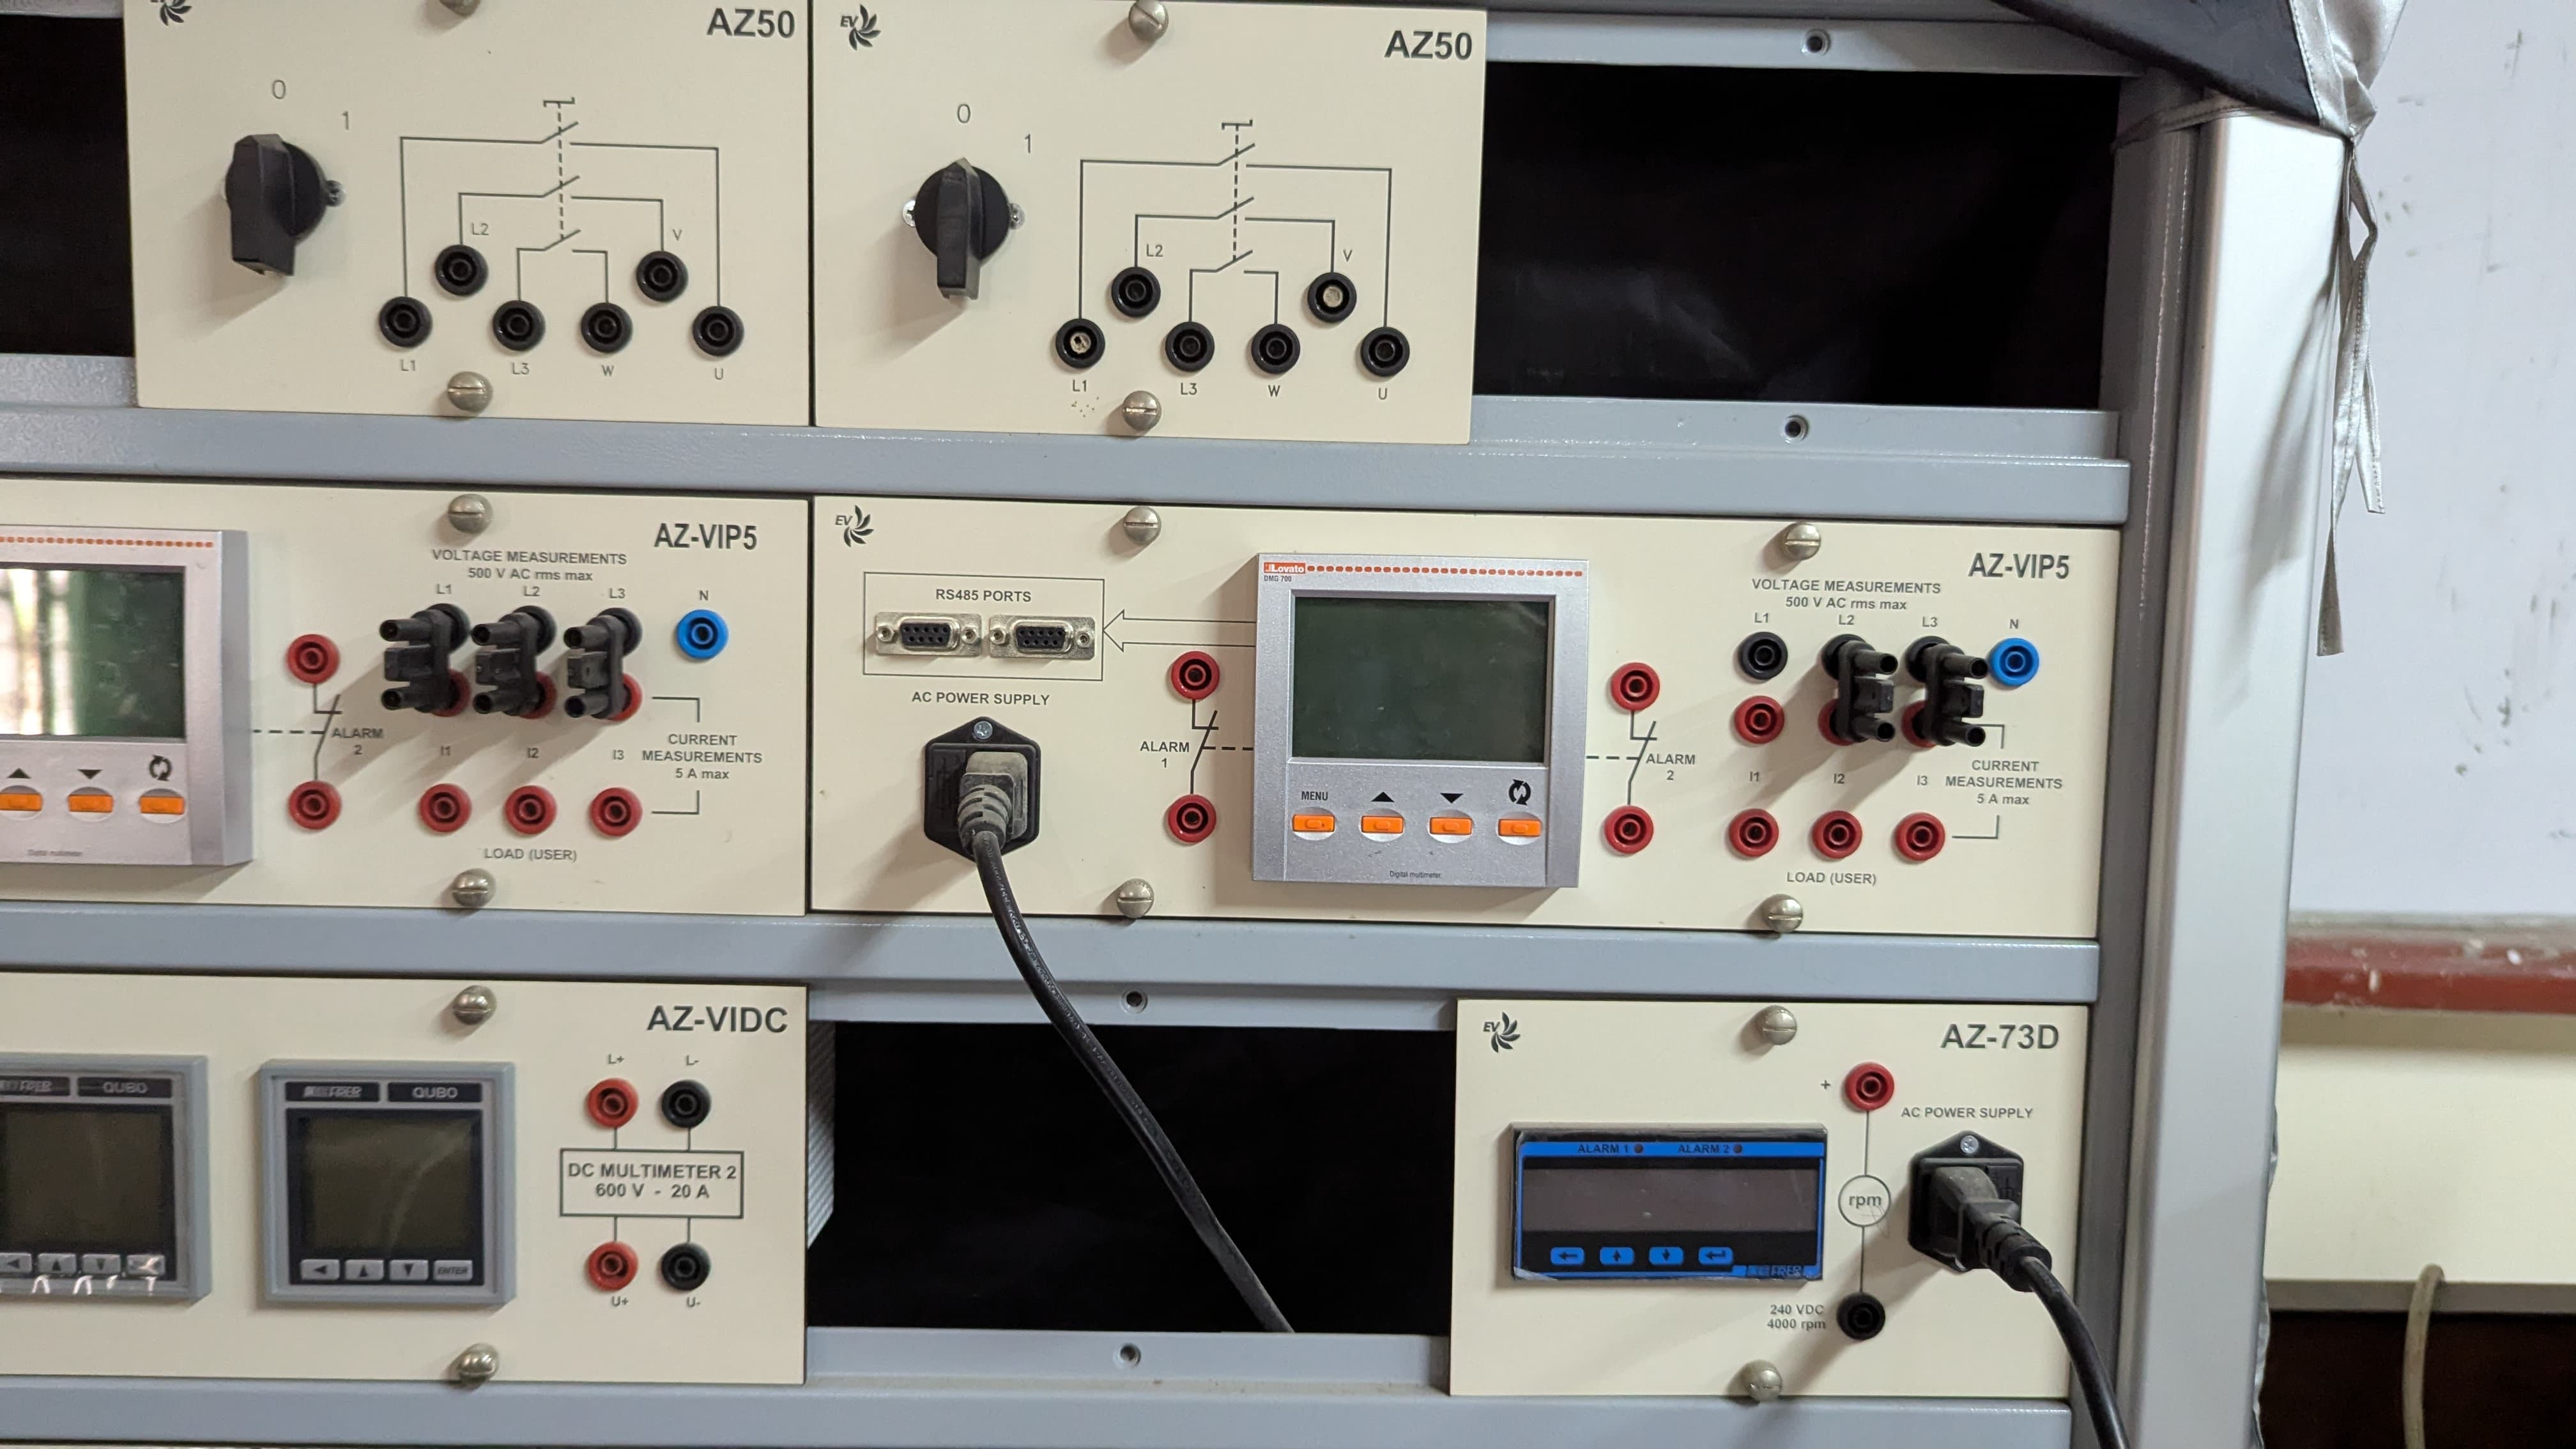
\includegraphics[width=1\linewidth]{Images/16}
			\caption{ }
		\end{subfigure}
		\hfill
		\begin{subfigure}[t]{.32\textwidth}
			\centering
			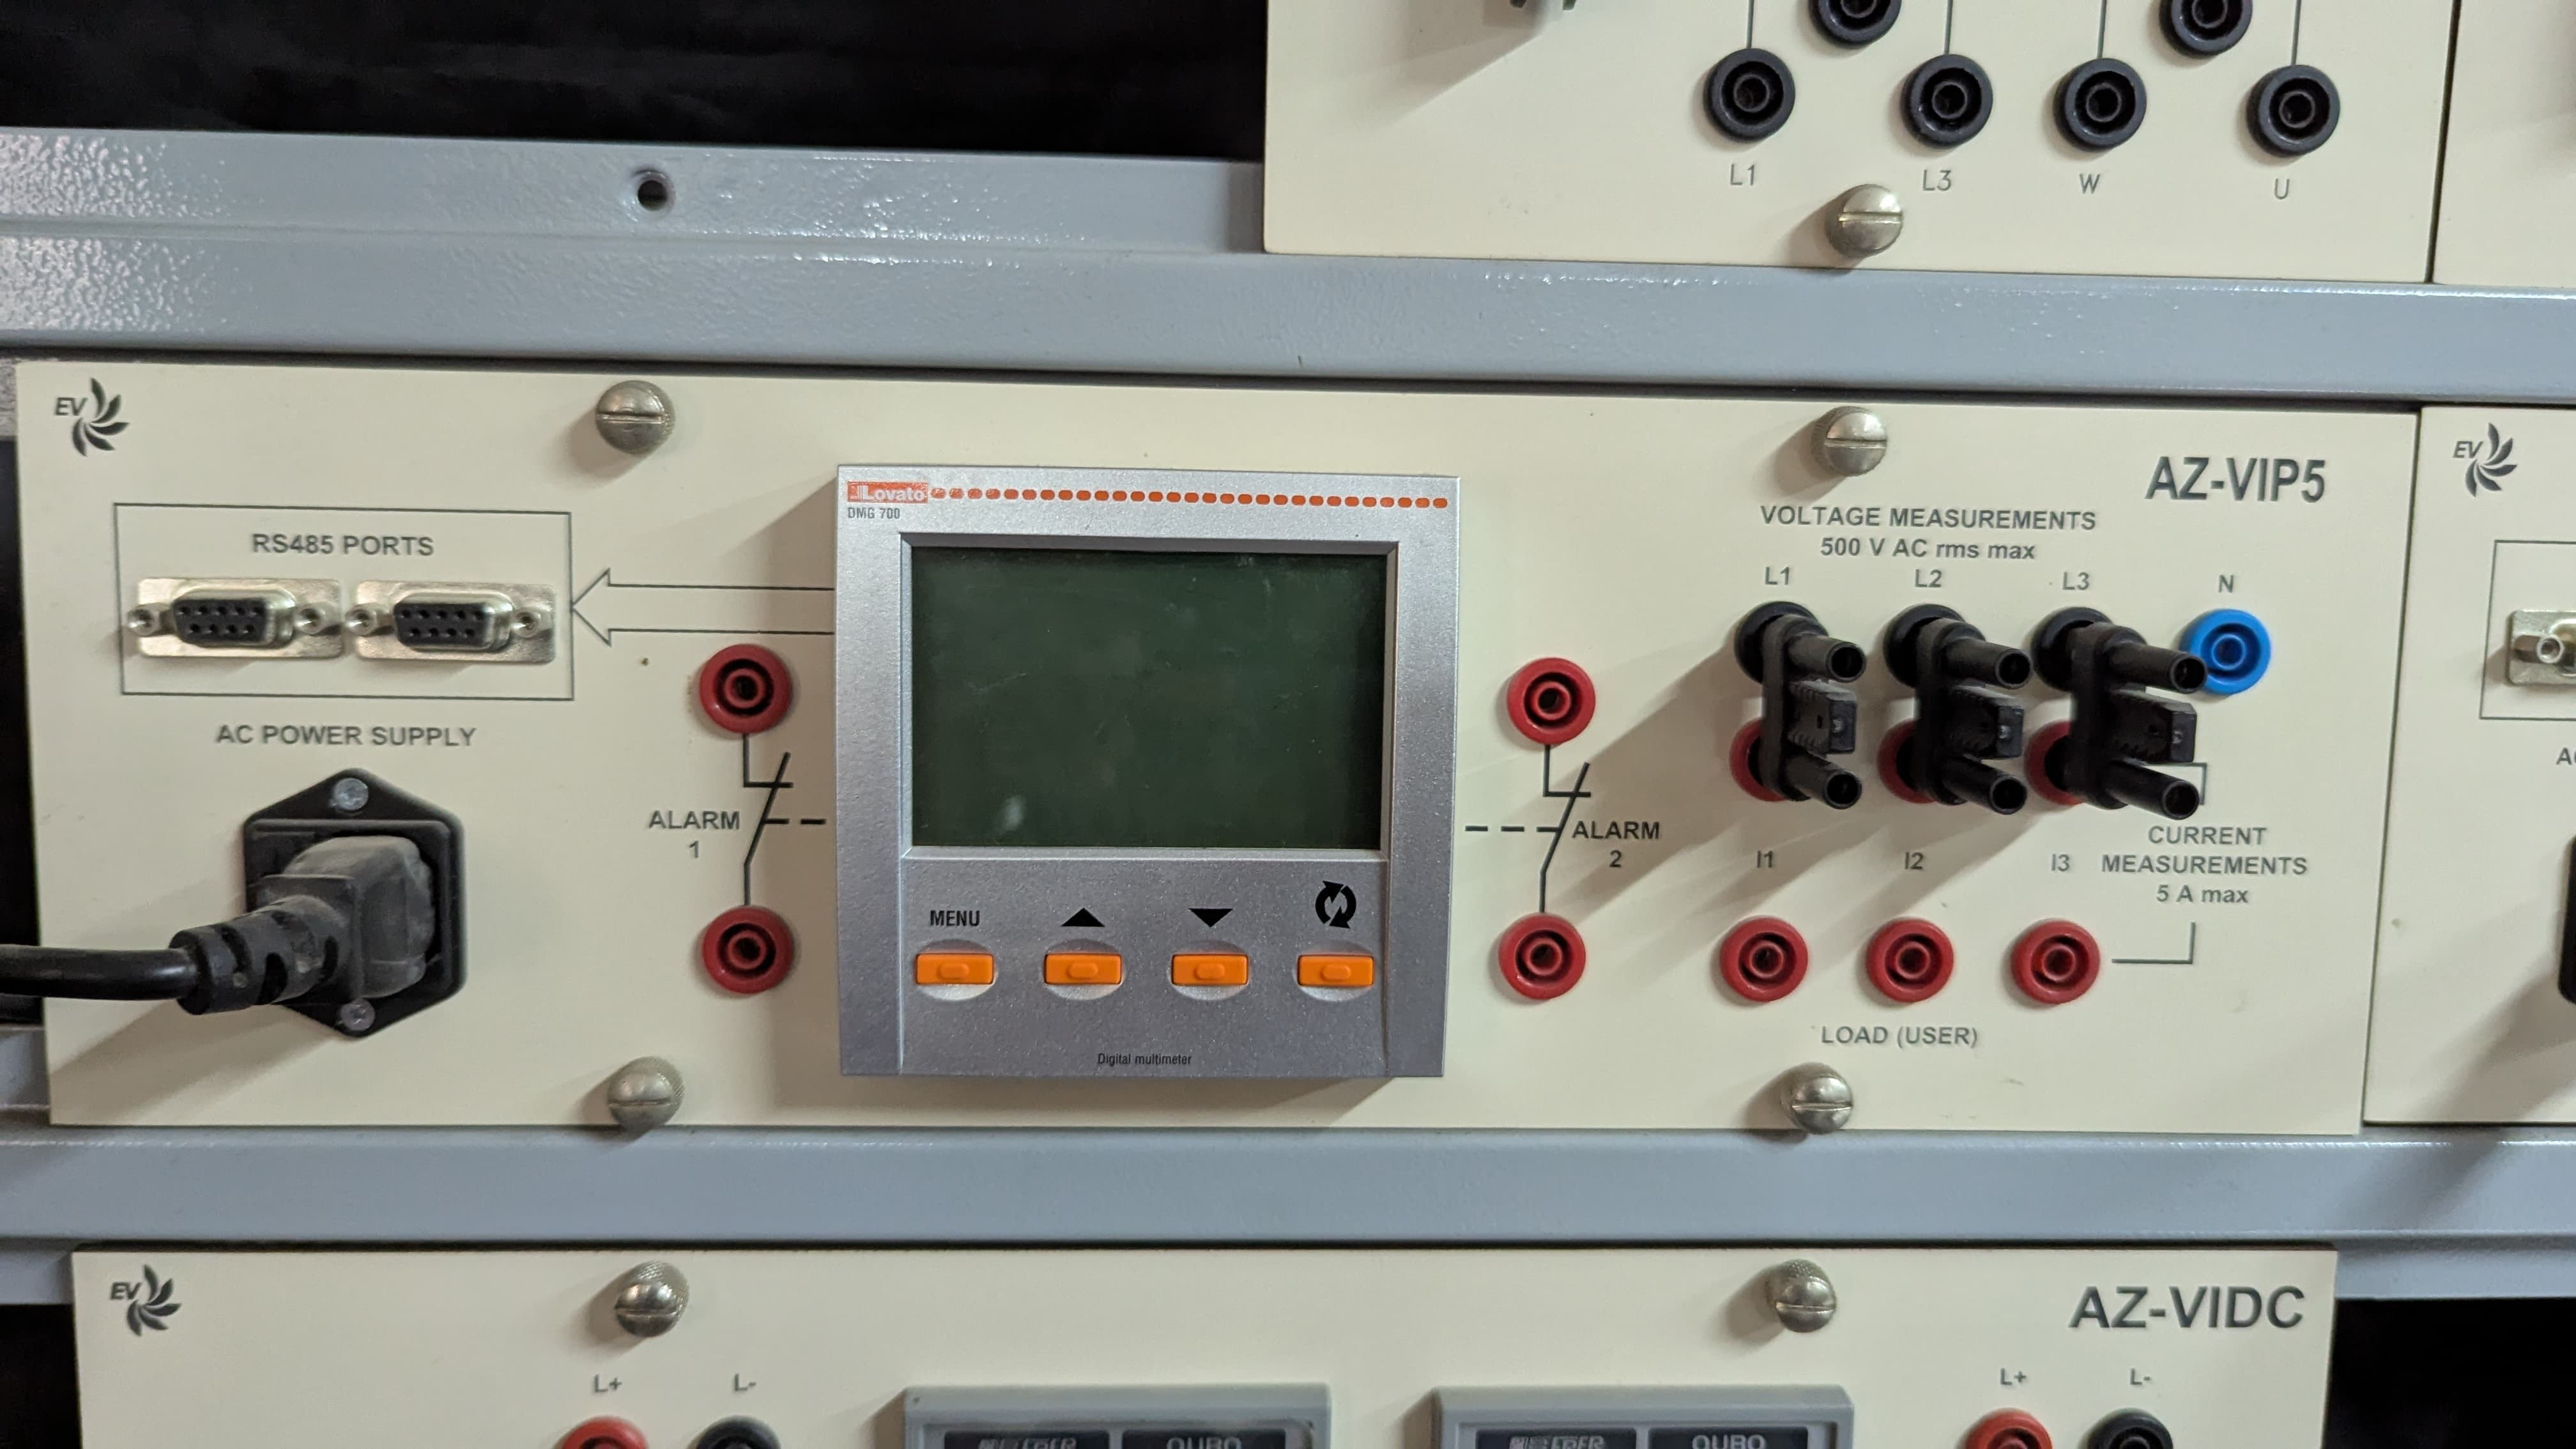
\includegraphics[width=1\linewidth]{Images/17}
			\caption{ }
		\end{subfigure}
	\end{figure}
	\begin{table}[H]
		\centering
		\caption{AC-DC Multimeter Specifications}
	\scalebox{.8}{
		\begin{tabular}{|l|c|c|}
			\hline
			\textbf{Feature} & \textbf{Specification} & \textbf{Notes} \\ \hline
			Modules & AZ50 (x2), AZ-VIPS (x2), AZ-VIDC, AZ-73D, AZ68, AZ67 & Modular components \\ \hline
			AZ50 Function & Basic Circuit Demo & \\ \hline
			AZ-VIPS Function & Digital Power Analysis & Voltage \& Current Measurement \\ \hline
			AZ-VIPS Voltage & 500V AC RMS Max & \\ \hline
			AZ-VIPS Current & 5A Max & \\ \hline
			AZ-VIPS Comm. & RS485 Ports & \\ \hline
			AZ-VIDC Function & DC Measurement & Two DC multimeters \\ \hline
			AZ-VIDC Meters & QUBO (x2) & Digital meters \\ \hline
			AZ-VIDC Range & 600V, 20A (DC) & For both multimeters \\ \hline
			AZ-73D Function & Digital Measurement & \\ \hline
		
			AZ67 Function & Connection/Switching & \\ \hline
			AZ67 Voltage & 36-400V (AC) & \\ \hline
			Connectivity & Banana Plugs & \\ \hline
			Power & AC Supply & Multiple Modules \\ \hline
			Construction & Rack Mounted Panels & \\ \hline
		\end{tabular}}
		
		\label{tab:modular_training}
	\end{table}
	
	
	\subsection{DC Current Stator}
	A DC current stator is a stationary part of a DC machine that produces a magnetic field necessary for the operation of the motor or generator.
		\begin{figure}[H]
		\centering
		\includegraphics[width=.4\linewidth, height=0.2\textheight]{"Images/14"}
		\caption{DC Current Stator}
	\end{figure}
	\begin{table}[H]
		\centering
		\caption{Specifications of current stator}
		\begin{tabular}{|l|c|}
			\hline
			\textbf{Feature} & \textbf{Specification} \\ \hline
			Type & DC Current Stator Training Module \\ \hline
			Manufacturer & EV \\ \hline
			Function & DC Motor/Generator Stator Connection Experiments \\ \hline
			Motor Types & DC (Separate, Shunt, Series, Compound), Universal, Repulsion \\ \hline
			Generator Types & DC (Separate, Shunt, Series, Compound), Inverse 3-Phase Alternator \\ \hline
			Connections & E1/F1, E2/F2, A1, A2, D1, D2, C1, C2, B1, B2, M, PE \\ \hline
			Indicator & Ground (PE) LED \\ \hline
		\end{tabular}
		\caption{DC Current Stator Training Module Specifications}
		\label{tab:dc_stator_module}
	\end{table}
	
	\subsection{Resistors}
	Resistors are passive electrical components that limit the flow of current in a circuit, helping in voltage regulation and circuit protection.
		
	\begin{figure}[H]
		\centering
		\begin{subfigure}[t]{.3\textwidth}
			\centering
			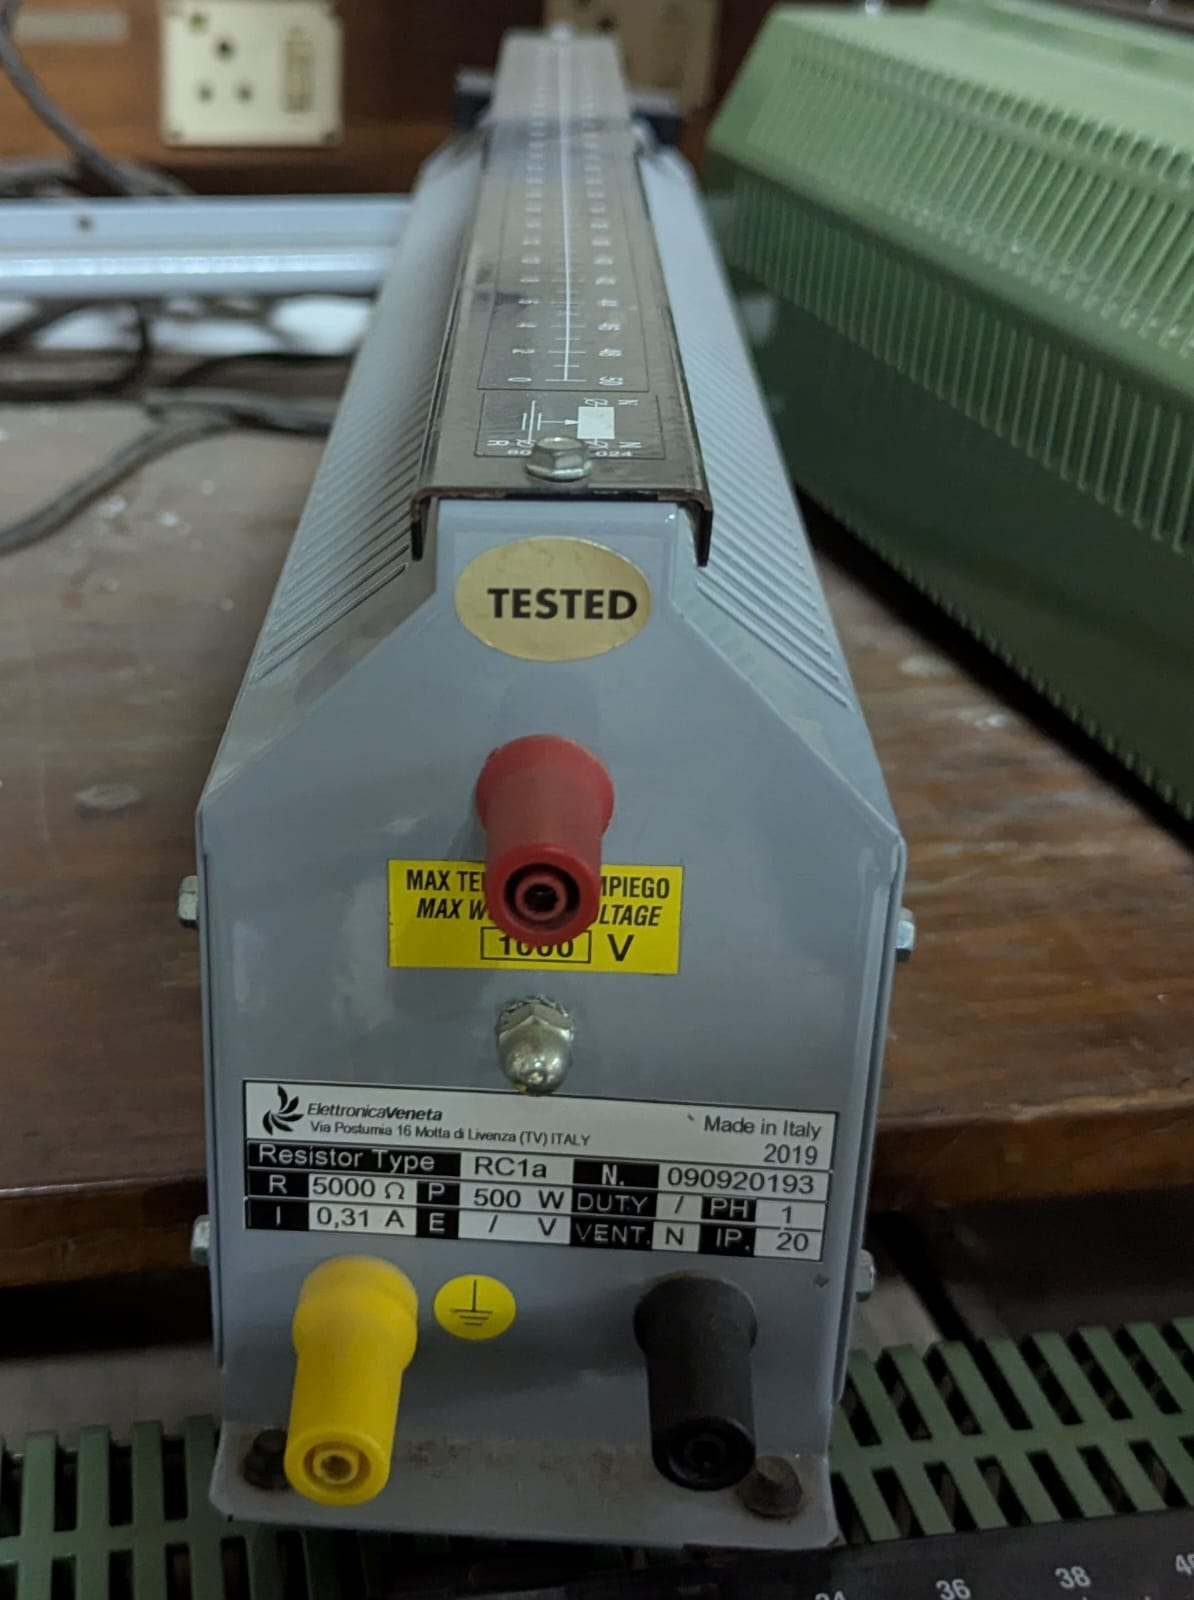
\includegraphics[width=.9\linewidth]{Images/10}
			\caption{ 5000$\Omega$ }
			\vspace{0.1cm}
		\end{subfigure}
		\hfill
		\begin{subfigure}[t]{.3\textwidth}
			\centering
			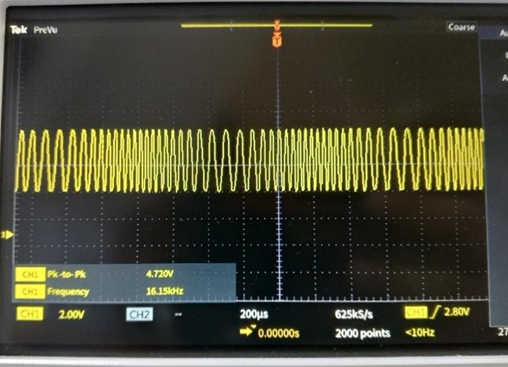
\includegraphics[width=.7\linewidth]{Images/11}
			\caption{  3$\times$50$\Omega$}
		\end{subfigure}
		\hfill
			\begin{subfigure}[t]{.3\textwidth}
			\centering
			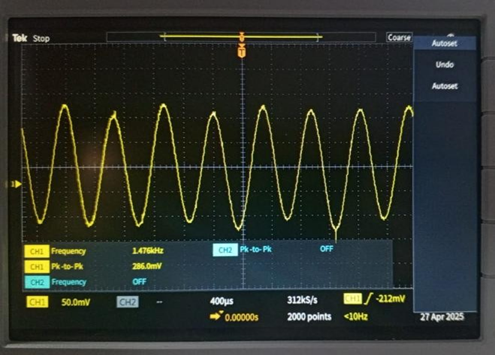
\includegraphics[width=1\linewidth]{Images/12}
			\caption{ 3$\times$50$\Omega$}
		\end{subfigure}
	\end{figure}
	\subsubsection{Specifications of Resistors}
	\begin{table}[H]
		\centering
		\caption{Resistors Specifications}
		\begin{tabular}{|l|c|c|c|c|c|}
			\hline
			\textbf{Resistance ($\Omega$)} & \textbf{Power (W)} & \textbf{Current (A)} \textbf{Max. Voltage (V)} & \textbf{Phase} & \textbf{IP} \\
			\hline
			50   & 500  & 3.16   & 1 & 20 \\
			200  & 500  & 1.58   & 1 & 20 \\
			5000 & 500  & 0.31   & 1 & 20 \\
			3 × 50  & 3 × 500  & 3 × 3.16   & 3 & 20 \\
			\hline
		\end{tabular}
	\end{table}
	\newpage
	\subsection{Power Supply}
	A 230V DC supply provides a stable direct current voltage for operating electrical machines and circuits requiring high voltage DC power.
			\begin{figure}[H]
			\centering
			\includegraphics[width=.45\linewidth, height=0.35\textheight]{"Images/3"}
			\caption{LCD/LED TV Trainer}
		\end{figure}
	\subsubsection{Specifications of Power Supply}
	\begin{table}[H]
		\centering
		\caption{Power Supply Specifications}
		\begin{tabular}{|l|c|}
			\hline
			\textbf{Specification} & \textbf{Details} \\ \hline
			Manufacturer & ElettronicaVeneta \\ \hline
			Model & AV-1/EV \\ \hline
			Input & 400V AC, 10A (Three-Phase) \\ \hline
			Variable AC Output & 0-430V AC (Three-Phase) \\ \hline
			Variable DC Output & 0-300V DC, 4A \\ \hline
			Fixed DC Outputs & 6V, 12V, 24V; 5V, 12V(2A); 220V(3A) \\ \hline
			Emergency Stop & Yes \\ \hline
		\end{tabular}
		
		\label{tab:power_supply}
	\end{table}
	\newpage
	\subsection{3-Point Starter}
	A 3-point starter is a protective device used to limit the inrush current when starting a DC motor, ensuring safe and efficient operation.
	
	\begin{figure}[H]
		\centering
		\begin{subfigure}[t]{.48\textwidth}
			\centering
			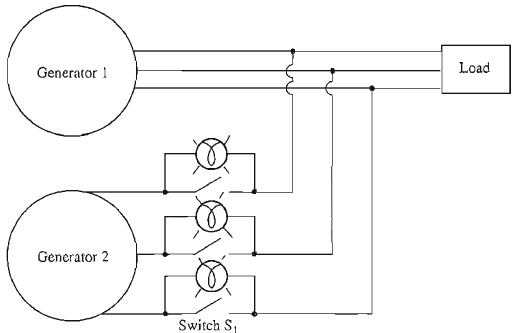
\includegraphics[width=.7\linewidth]{Images/1}
			\caption{ 3-Point Starter }
			\vspace{0.1cm}
		\end{subfigure}
		\hfill
		\begin{subfigure}[t]{.48\textwidth}
			\centering
			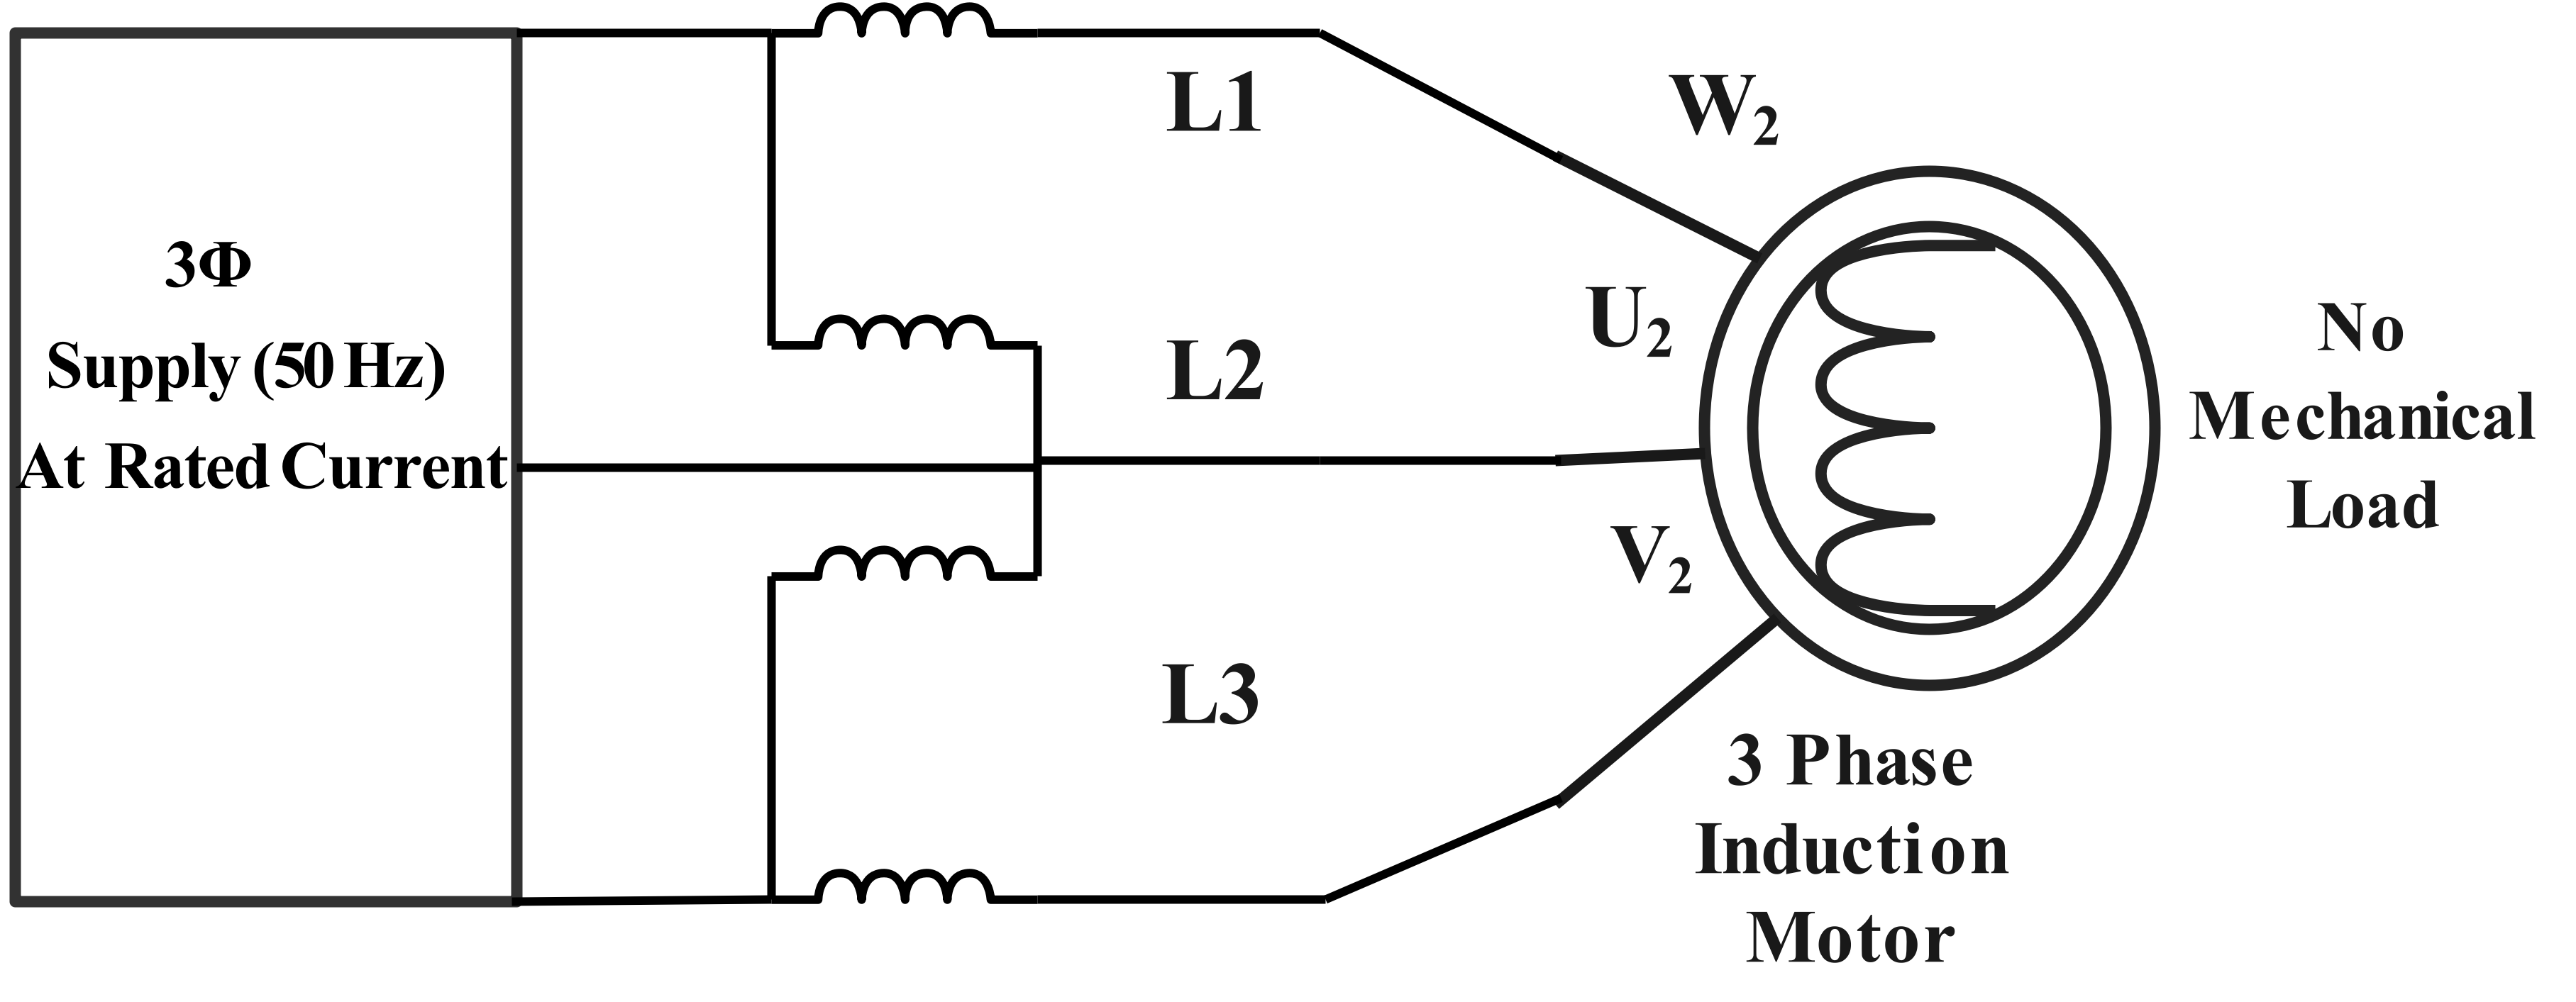
\includegraphics[width=1\linewidth]{Images/2}
			\caption{Motor-Starter Circuit Connector}
		\end{subfigure}
	\end{figure}
	
	\section{Safety and Precautions}
	Handling electrical machines requires adherence to safety guidelines to prevent electrical hazards, injuries, and equipment damage. Some key precautions include:
	\begin{enumerate}
		\item Always wear insulating gloves and shoes while working with electrical machines.
		\item Ensure proper grounding and insulation to avoid electrical shocks.
		\item Avoid touching live wires and rotating parts while machines are operational.
		\item Regularly inspect machines for loose connections and overheating.
		\item Follow manufacturer guidelines and safety procedures during operation and maintenance.
	\end{enumerate}
	

	


	
	
	
	
	
	
	
	
	\section{Discussion}
	
During the experiment, the specifications and photographs of various electrical components and training modules were carefully noted. The equipment was examined to understand its operational parameters, including voltage, current, and power ratings. Each component’s function was identified, and its role in the training system was documented.
Safety precautions were strictly followed throughout the experiment. Proper handling of high-voltage equipment was ensured, and insulated tools were used to prevent accidental shocks. Additionally, connections were double-checked before powering the system to avoid short circuits or incorrect wiring. Personal protective equipment was worn, and the workspace was kept organized to minimize hazards.
The data collected provided insight into the technical specifications of the equipment, which will be useful for future experiments and practical applications.
	
	
	
\end{document}
